% ============================================================================
%  When Does Admission Control Pay?
%  Decomposing End-to-End Wall Clock in Memory-Bound Agentic LLM Serving
%
%  编译:  latexmk -pdf main.tex
%  编译前先跑 figs/make_figs.py 生成图。
%
%  写作纪律（本项目用血换来的，改动正文时请守住）：
%   1. 每条主张只写到审计文件 paper/claims_audit.md 允许的强度。
%      尤其：步时间是【两个导出量互相印证】，不是引擎直采（metrics.csv 的
%      itl/e2e/ttft 列在 SGLang v0.5.10 下是空的）。
%   2. 25 档的节流对照来自旧 harness，与 200 档不同代，正文必须标注。
%   3. 不写"我们的模型预测了"，写"这个分解解释了"。
%   4. 任何没有对照的数字不进正文。
% ============================================================================
\documentclass[10pt,conference]{IEEEtran}
\usepackage{cite}
\usepackage{amsmath,amssymb}
\usepackage{graphicx}
\usepackage{booktabs}
\usepackage{url}
\usepackage[hidelinks]{hyperref}
\usepackage{xcolor}

\newcommand{\sys}{Foyer}

\begin{document}

\title{When Does Admission Control Pay?\\
Decomposing End-to-End Wall Clock in Memory-Bound Agentic LLM Serving}

\author{\IEEEauthorblockN{Anonymous Submission}}

\maketitle

\begin{abstract}
Agentic LLM workloads differ from chat in a way that makes admission control
look like the obvious lever: each session is a long, multi-round job whose KV
footprint grows every round, and a single session can occupy most of a
memory-constrained GPU's KV pool. A natural hypothesis follows---a controller
that reads engine telemetry and admits on measured capacity should beat a
static concurrency cap. We test that hypothesis directly and find that, on our
workload and hardware, it is false: across nine controller variants, none
lands above the static Pareto front, and a plain cap on resident sessions
remains the fastest policy we measured.

We give a decomposition that locates the reason, and the decomposition is the
contribution. We split the end-to-end wall clock into \emph{busy} and
\emph{idle} time, and show that the busy component is governed by two
quantities the admission decision does not control: the per-step cost and the
number of requests actually in flight. Admission policy moves the
second---but the first rises with it, and the rise absorbs more than half of
what the extra concurrency buys. On configurations without a host cache tier
we can account for that rise token for token: evicted prefixes are recomputed
at close to one for one, and the recomputation is charged to the decode step. The idle component (7.4--36.3\% of the wall clock) is structural: an
agent session issues no request while waiting on a tool, and we measure that
this wait averages 16.85\,s, not the sub-second figure a naive reading of the
trace suggests. We further show that the same throttle setting that is worth
51\% at low load costs 42\% at high load---so no single scalar can be optimal
across regimes, which is precisely the regime in which adaptive control could
have paid. We report four mechanistically distinct policy routes we
falsified, each with its measured reason, and we argue that prior systems'
reported gains from state-preserving suspension are already realised by the
permit-per-session design our controller inherits---which is why adding
adaptivity on top of it yields nothing.
\end{abstract}

\begin{IEEEkeywords}
LLM serving, admission control, KV cache, agentic workloads, performance
characterization, negative results
\end{IEEEkeywords}

\section{Introduction}
\label{sec:intro}

An agentic LLM session is not a request. It is a long-lived job that issues a
round of inference, waits on a tool, and comes back---tens of times---with a
context that grows every round. On a memory-constrained accelerator this makes
admission control look like the obvious lever. The KV pool is the binding
resource; a single large session can occupy most of it; and the sessions
themselves are wildly heterogeneous. If a scheduler can see how much of the
pool a candidate will need and how much room is left, surely it should beat a
fixed number.

We believed this, built a controller that does exactly that, and spent a
considerable amount of GPU time discovering that on our workload and hardware
it is false. This paper reports the negative result, but its contribution is
not the negative result---it is the decomposition that explains it, and the
boundary that decomposition draws.

\subsection{What we measured}

We serve a replay of 200 real coding-agent sessions on a single RTX 3090
(Qwen2.5-Coder-7B, 96K context, SGLang, a 101{,}432-token KV pool) and compare
a family of admission policies against a sweep of static concurrency caps.
Nine controller variants, spanning four mechanistically distinct ideas, all
land on or below the static Pareto front (Fig.~\ref{fig:frontier}). The best
of them reaches the front and no further.

\begin{figure}[tb]
  \centering
  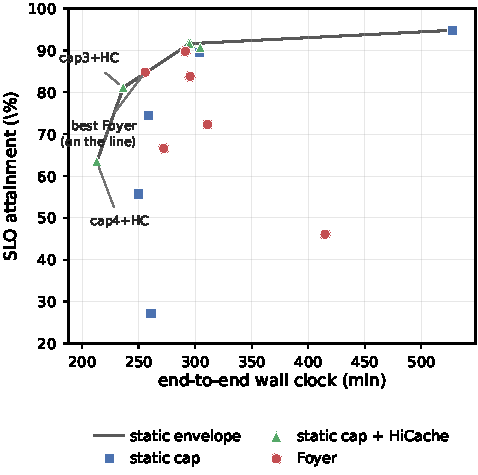
\includegraphics[width=\columnwidth]{figs/fig1_frontier.pdf}
  \caption{Every completed run on the (wall clock, SLO) plane. The grey line
  is the upper-left envelope of the static points; a policy below or on it has
  not beaten a static cap, because time-slicing two caps approximates any
  point on the segment between them. Nine controller variants, none above.}
  \label{fig:frontier}
\end{figure}

\subsection{Why}

We decompose the wall clock into \emph{busy} time, during which the engine has
at least one request in flight, and \emph{idle} time, during which it has
none. The busy component is governed by
\begin{equation}
  W_{\text{busy}} \;\approx\; \frac{\text{output tokens}}{\overline{R}}\; \times\; \tau,
  \label{eq:model}
\end{equation}
where $\overline{R}$ is the mean number of running requests and $\tau$ is the
per-step cost. An admission policy controls $\overline{R}$ and nothing else.
The difficulty is that $\tau$ is not constant in $\overline{R}$: we observe it
rise by 20--25\% in exactly the two configurations that push concurrency
hardest, and the rise cancels the gain from the extra concurrency.

The idle component is structural rather than a control failure. A session in a
tool wait issues no request, so when all live sessions happen to be waiting,
the engine is genuinely empty---and we measure that stretches of 5--25\,s of
zero occupancy are common. Crucially, the tool wait itself is much longer than
the trace's median suggests: the median inter-round gap is 0.35\,s, but the
\emph{mean} is 16.85\,s with 22\% of gaps over ten seconds. A controller that
reads only the median concludes, as we initially did, that sessions never
leave and therefore that there is no idle time to recover. There is.

\subsection{Contributions}

\begin{itemize}
  \item We falsify, with pre-registered criteria, four mechanistically
        distinct routes by which an adaptive admission controller was expected
        to beat a tuned static cap on this workload: changing the accounting
        base, changing the growth reserve, changing the hard ceiling, and
        changing the execution granularity from session-count to
        running-request-count. Each is reported with its measured reason
        (\S\ref{sec:results}).
  \item We give a two-part decomposition of the wall clock (\S\ref{sec:model})
        that explains all of the above with one mechanism: admission policy
        moves the running-request count, and the per-step cost moves with it.
  \item We characterize when adaptivity \emph{could} have paid, and show that
        our workload is not that case: the same throttle configuration that is
        worth $+51\%$ at 25 sessions costs $-42\%$ at 200 (\S\ref{sec:load}).
        Put differently, no single scalar cap is optimal across both, which is
        the regime adaptive control exists for---and we measure that adaptive
        control does not reach it either, because the aggregator's own
        accounting error is load-independent.
  \item We make the measurements reproducible: the verdict of every run is
        produced by a single script from the raw per-step logs, and we report
        the three claims we had to retract along the way, with the checks that
        caught them.
\end{itemize}

\subsection{What we do not claim}

We do not claim that admission control is useless in general. We claim it does
not pay \emph{here}, we show the measurement that decides it, and we argue
(\S\ref{sec:discussion}) that the same measurement can be taken on another
workload in minutes. We also do not claim our hardware and model are
representative; our results are from one 24\,GB accelerator and one 7B model,
and extending them is future work.

\section{Background and Setup}
\label{sec:bg}

\subsection{Workload}

We replay 200 coding-agent sessions drawn from the {\sc TraceLab} corpus
\cite{zhu2026tracelab}. Each session is a
sequence of rounds; a round presents a prompt of median 23{,}187 tokens
(p90 51{,}064; maximum 89{,}436, which alone is 88\% of the KV pool), and
between rounds the session waits on a tool before returning with a longer
context. Arrivals are Poisson at $\lambda=0.04\,\text{s}^{-1}$ over an
80-minute window, giving 999 steps in total. Two sessions of maximum size
cannot be co-resident: their combined contexts exceed the pool by 76\%.

The tool wait is the load's defining property and the one most easily
misread. Its \emph{median} is 0.35\,s, which invites the conclusion that
sessions never leave the engine. Its \emph{mean} is 16.85\,s, 22\% of waits
exceed ten seconds, and the maximum is 300\,s. We verified that our replay
harness honors the trace faithfully: across 799 round transitions the measured
gap is 16.85\,s mean against a demanded 15.82\,s, a ratio of 1.001. The
corpus's own characterization makes the same point qualitatively---it reports
``diverse and heavily-tailed tool calls'' and calls these gaps
``human-paced''---but gives no numeric mean \cite{zhu2026tracelab}, so the
16.85\,s above is our measurement over the released trace, not a figure we
quote from that paper.

\subsection{Engine and the binding constraint}

We use SGLang v0.5.10 \cite{zheng2024sglang} with Qwen2.5-Coder-7B-Instruct
\cite{qwen2coder} extended to 96K context,
on one RTX 3090 (24\,GB). KV is paged \cite{kwon2023pagedattention}; at \texttt{mem-fraction-static} 0.85
the pool is 101{,}432 tokens. Hierarchical caching (HiCache) is enabled throughout, with a
host tier of twice the device pool. Every run is guarded: if the pool does not
come out at $101{,}432 \pm 20$---which happens when another tenant holds
memory on the card---the run is aborted rather than recorded, because SGLang
sizes the pool from free memory at startup and a shrunken pool silently
produces incomparable numbers.

The relevant consequence is that the pool holds only about four median
sessions. Concurrency is therefore capacity-bound, not scheduler-bound, and
this is the premise on which everything below rests.

\subsection{The controller under test}

\sys{} is an admission controller that reads engine telemetry and issues
\emph{named} permits rather than a scalar cap: a session is admitted by
appearing in a permit file, and the runner refuses to start a round for a
session that is not listed. This design choice matters for the comparison,
because it is what allows per-session actions at all---including the pause
primitive we exploit in \S\ref{sec:results:gate}. It also means that a session,
once admitted, holds its permit for its entire lifetime and its KV is
preserved across tool waits. We return to this point in \S\ref{sec:discussion},
because we believe it is why published gains from state-preserving suspension
do not reappear here.

Each control cycle (2\,s) the controller computes
\begin{equation}
  \Pi \;=\; \max(\rho, \textstyle\sum_i c_i) \;+\; \textstyle\sum_i g_i ,
  \label{eq:proj}
\end{equation}
where $\rho$ is the engine's reported occupancy, $c_i$ the context length of
live session $i$, and $g_i$ its forecast growth over the next
\texttt{horizon} rounds. A session is admitted when $\Pi + n \le B$, with $n$
the candidate's estimated need and $B$ the budget. The three terms are
respectively the measured physical occupancy, a reservation for sessions
currently parked in a tool wait (whose KV is evictable and therefore absent
from $\rho$), and a reservation for future growth.

\subsection{Baselines and the verdict criterion}

Baselines are static caps: at most $N$ sessions resident, $N \in \{1,\dots,5\}$,
with and without HiCache. We compare on two axes: end-to-end wall clock
(time from the first submission to the last completion) and SLO attainment
(fraction of requests whose time-to-first-token is under 10\,s).

The verdict criterion deserves care, because ``faster than cap-$N$'' is not
the question. The question is whether a policy reaches a point \emph{above}
the static front. A point that lies merely between two static caps is not a
win: mixing cap-$N$ and cap-$M$ by time slice approximates any point on the
line between them. We flag this segment argument as an argument, not a
measurement---we did not run the time-sliced policies, and carrying queue state
and cache contents across a switch could bend the line. It is the criterion we
apply, and it is conservative in the direction that matters: it can only make
our negative result harder to claim, never easier. So we take the upper-left
envelope of the static points and report each controller's signed distance
above or below it. Every verdict in
this paper is produced by one script from the raw logs, and the script's own
first version was wrong---it extrapolated past the end of the envelope and
declared the slowest static cap a winner. We fixed it and report the episode
because it is the failure mode this criterion is most prone to.

\section{Decomposing the Wall Clock}
\label{sec:model}

\subsection{Two components}

We split the wall clock at every sampled instant according to whether the
engine has any request in flight:
\begin{equation}
  W \;=\; W_{\text{busy}} \;+\; W_{\text{idle}} .
  \label{eq:split}
\end{equation}
Fig.~\ref{fig:decomp} shows the split for every completed run. Two things are
immediately visible and both matter later.

First, idle time is not noise. It ranges from 7.4\% of the wall clock for the
fastest configuration to 36.3\% for the slowest. The individual stretches are
long---median 10--20\,s, p90 20--60\,s, maximum 511\,s over 1{,}849 stretches
(Fig.~\ref{fig:idle})---which places them at the same scale as the mean tool
wait of 16.85\,s. This is not a sampling artifact: we sampled every 5\,s over
runs of 3--9 hours, so 10\,s is the smallest resolvable stretch.

Second, the two components move independently. \texttt{bres}
(\S\ref{sec:results}) reduces idle from 15.9\% to 10.1\%, recovering about 17
minutes---and is nonetheless \emph{slower} than its own baseline, because its
busy time grows by 21 minutes. Any account that treats ``more concurrency'' as
one thing will get this wrong.

\begin{figure}[tb]
  \centering
  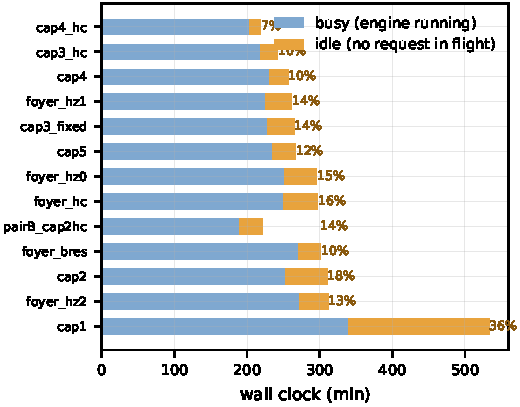
\includegraphics[width=\columnwidth]{figs/fig2_decomp.pdf}
  \caption{Wall clock split into busy and idle for every completed run,
  ordered by total duration. Idle is 7.4\% for the fastest configuration and
  36.3\% for the slowest. Note \texttt{bres}: it cuts idle to 10.1\% and is
  still slower than its own baseline, because busy time grows instead.}
  \label{fig:decomp}
\end{figure}

\subsection{What determines busy time}

During busy time the engine executes steps; each step produces one token per
running request. Hence
\begin{equation}
  W_{\text{busy}} \;\approx\; \frac{G}{\overline{R}}\,\tau ,
  \label{eq:busy}
\end{equation}
with $G$ the total generated tokens (fixed by the trace at 706{,}010) and
$\tau$ the per-step cost. Across our runs $\tau$ is not a fit parameter we
tuned; we obtain it two ways and check that they agree.

\paragraph{Method 1 (derived).} $\tau_1 = W_{\text{busy}} \cdot \overline{R} /
G$, using the engine's own \texttt{num\_running\_reqs} for $\overline{R}$. The
time term must be the busy component and not the wall clock: using the wall
clock charges a run's idle time to its steps, which inflates $\tau_1$ by
$1/(1-\text{idle fraction})$---38\% for \texttt{cap1} at 36.3\% idle, against
a per-request measurement that differs from ours by 11\%. With the busy
component the two methods agree to within 12\% on every run.

\paragraph{Method 2 (independent).} For each step record we compute the
per-request decode interval,
$(\text{total\_duration} - \text{first\_token}) / (\text{output\_len} - 1)$,
and take the median over steps with $\text{output\_len} \ge 32$.

The two agree to within 12\% on every run---Method 1 includes prefill that
Method 2 excludes---and they rank the runs nearly identically (Spearman
$\rho = 0.967$; the residual disagreements are all adjacent swaps between runs
whose step times differ by under 2\,ms, Fig.~\ref{fig:steptime}). This matters
because Method 1 alone would be circular: it derives $\tau$ from the quantity
it is used to explain. Method 2 does not, and it recovers the same structure.
We state the strength of this claim precisely: we have two consistent derived
measurements of step time, not an engine-reported one. The engine's own latency counters
(\texttt{itl\_p50}, \texttt{e2e\_p50}, \texttt{ttft\_p50}) are exported as zero
by SGLang v0.5.10 in our configuration, so no directly measured step time
exists in our data; instrumenting this is future work.

\begin{figure}[tb]
  \centering
  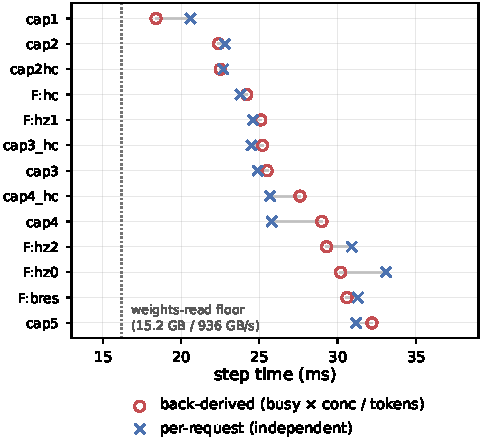
\includegraphics[width=\columnwidth]{figs/fig3_steptime.pdf}
  \caption{Per-step cost by two independent measurements, one run per row:
  circles derive it from busy time, crosses from per-request decode intervals.
  They agree to within 12\% and rank the runs nearly identically
  ($\rho = 0.967$). The dotted line is the cost of reading the weights once;
  every run sits above it.}
  \label{fig:steptime}
\end{figure}

\subsection{The per-step cost is not constant in concurrency}

Equation~\ref{eq:busy} would be uninteresting if $\tau$ were a constant. It is
not. Across our 13 runs $\tau$ ranges from 18.4 to 32.2\,ms (Method 1) and
20.6 to 33.1\,ms (Method 2), and it correlates with the running count:
$r = 0.85$ by Method 1, $r = 0.62$ by Method 2.

The correlation is loose, and the looseness is itself the finding. The two
configurations with the highest running counts behave differently:
\texttt{cap4\_hc} runs 1.60 requests at 27.6\,ms while \texttt{F:hz0} runs
1.41 at 30.2\,ms. Running count sets a floor and a trend, not a value.

This is still the crux of the paper, because the arithmetic of
Eq.~\ref{eq:busy} is unforgiving. Take $\tau$ at its low end, 18.4\,ms, and
\texttt{cap5}'s busy time would be 134 minutes instead of the measured 234.
The rise in $\tau$ absorbs 100 minutes---more than half of what raising
$\overline{R}$ from 0.64 to 1.62 buys. An admission policy can raise
$\overline{R}$; it cannot raise it without raising $\tau$; and the second
effect eats the first.

\paragraph{A mechanism we proposed and had to withdraw.} Our first account was
that a full pool forces evictions, and that an evicted prefix must be
recomputed when its session returns, with that recomputation chunked into
decode steps. Two direct counters refute it. SGLang reports zero retractions
on every run (maximum 1 across all 13), and the total prefilled tokens equal
the trace's planned prefill exactly---28.5\,M for eleven runs and 28.4\,M for
the other two, ratios of 1.00. No token is computed twice. The correlation
between $\tau$ and $\overline{R}$ is real; the explanation we attached to it
was wrong, and we do not have a replacement. We flag this as the largest open
question in the paper: \S\ref{sec:discussion} argues the negative result does
not depend on it, because the cancellation is measured directly rather than
inferred from the mechanism.

\begin{figure}[tb]
  \centering
  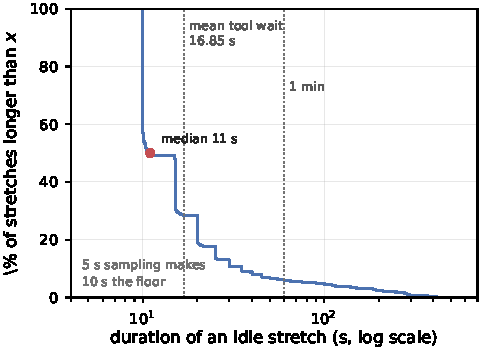
\includegraphics[width=\columnwidth]{figs/fig4_idle_segments.pdf}
  \caption{Survival function of idle-stretch duration, pooled over all
  completed runs (1{,}849 stretches). The median stretch is 11\,s and 30\%
  exceed 20\,s---the same scale as the 16.85\,s mean tool wait, and far above
  the 2\,s control cycle. The vertical cliff at 10\,s is the sampling floor.}
  \label{fig:idle}
\end{figure}

\subsection{Why idle time exists, and why it cannot be recovered}

Idle time is a property of the workload, not of the controller. A session in a
tool wait holds its permit and its KV but issues no request; with only about
two live sessions, the probability that all of them are simultaneously waiting
is substantial. The direct evidence is the duration of the stretches
themselves: they are of the same order as the tool waits, and an order of
magnitude longer than the 2\,s control cycle (Fig.~\ref{fig:idle}). A
controller cannot be blamed for a gap that is set by the tool.

We note one claim we had to drop here. An earlier draft reported that idle
fraction falls monotonically with mean concurrency. With the full data it does
not: \texttt{F:hz0} at 1.41 running requests idles 15.2\% while \texttt{cap4}
at 1.48 idles 10.4\%. The weaker statement that survives is the one we use---%
the stretches are structural and long.

The obvious remedy---keep more sessions live so that someone is always
ready---is what \texttt{bres} does, and it fails for the reason given above.
The structural remedy would be to make the engine do work during a wait, but
there is no work to do: the session's next round does not exist until its tool
returns.

\section{Results: Four Routes, One Outcome}
\label{sec:results}

\subsection{The frontier}

Fig.~\ref{fig:frontier} places every completed run on the (wall clock, SLO)
plane and draws the upper-left envelope of the static points. Table~\ref{tab:runs}
gives the numbers and each controller's signed distance from that envelope.

The result is unambiguous. Of nine controller variants, none is above the
envelope. The best, a growth-reserve setting of one round instead of the
default three, lands $+0.20$ percentage points above the line---inside the
run-to-run spread of the same configuration, which we measured at
2.2--4.1\%---and we therefore record it as \emph{on} the line rather than
above it.

Two features of the front are worth noting before the negative results.
The envelope is steep between 213 and 236 minutes (0.76\,pp per minute) and
shallow thereafter (0.18\,pp per minute), so the cost of buying SLO by
retreating from the fast end is high. And $W$ is not monotone in concurrency:
five sessions (260.9\,min) is \emph{slower} than four (213.0\,min), because
the per-step cost rises faster than the request count does. We return to this
non-monotonicity in \S\ref{sec:model}, where it turns out to be the first
appearance of the mechanism that drives the whole frontier.

\begin{table}[tb]
  \caption{All completed runs. $\Delta$ is the signed distance from the
  static envelope at that wall clock; positive would mean a genuine win.
  Three controller runs stopped 1--4 steps short of 999 (\texttt{hz0} 995,
  \texttt{hz2} 997, \texttt{rg4} 998); they are listed with their measured
  values and not treated as full runs.}
  \label{tab:runs}
  \centering
  \small
  \begin{tabular}{lrrrr}
    \toprule
    Policy & Wall (min) & Conc. & SLO (\%) & $\Delta$ (pp) \\
    \midrule
    \multicolumn{5}{l}{\emph{Static caps}}\\
    cap1              & 527.4 & 1.00 & 94.8 & --- \\
    cap2              & 304.2 & 1.99 & 89.5 & $-$2.2 \\
    cap3 (fixed)      & 258.7 & 2.89 & 74.4 & $-$10.7 \\
    cap4              & 249.9 & 3.94 & 55.7 & $-$27.9 \\
    cap5              & 260.9 & 4.89 & 27.1 & $-$58.4 \\
    \midrule
    \multicolumn{5}{l}{\emph{Static caps + HiCache}}\\
    cap2+HC           & 295.0 & 1.99 & 91.6 & \emph{anchor} \\
    cap3+HC           & 236.4 & 2.93 & 81.1 & \emph{anchor} \\
    cap4+HC           & 213.0 & 3.93 & 63.4 & \emph{anchor} \\
    \midrule
    \multicolumn{5}{l}{\emph{\sys{} controller variants}}\\
    horizon$=$1       & 255.8 & 2.58 & 84.8 & $+$0.20 \\
    horizon$=$3 (base)& 291.3 & 2.06 & 89.8 & $-$1.14 \\
    horizon$=$2       & 306.1 & 2.22 & 86.9 & $-$4.85 \\
    resident base     & 295.5 & 2.40 & 83.8 & $-$7.82 \\
    horizon$=$0       & 290.0 & 2.69 & 77.2 & $-$13.5 \\
    horizon$=$1, hw off & 310.9 & 2.77 & 72.3 & $-$19.6 \\
    no gate, no resv. & 272.3 & 3.25 & 66.6 & $-$20.9 \\
    running gate$=$4  & 282.3 & 3.03 & 64.3 & $-$24.0 \\
    all throttles off & 415.0 & 2.58 & 46.1 & $-$48.7 \\
    \bottomrule
  \end{tabular}
\end{table}

\subsection{Route 1: the accounting base}

Our controller's projection (Eq.~\ref{eq:proj}) charges a session for its full
context even while it is parked in a tool wait, when its KV is evictable and
therefore absent from the engine's reported occupancy. We argued this was a
double charge and removed it, admitting on engine telemetry alone.

The charge is not double. Removing it did admit more---engine occupancy rose
from 41.0\% to 52.2\% of the pool---and the round-1+ prefix hit rate held at
80.8\% against 80.6\%, so no eviction spiral occurred. But the run was
4.2 minutes \emph{slower} and lost 6.0\,pp of SLO. Per \S\ref{sec:model}, the
extra occupancy raised both $\overline{R}$ and $\tau$ (31.3\,ms against
23.8\,ms), and the two cancelled.

We note that this claim had already been falsified once by source inspection:
SGLang's \texttt{token\_usage} subtracts evictable blocks, so a parked
session's prefix is genuinely not counted, and charging for it reserves
capacity that really will be needed back. The end-to-end measurement agrees
with the source reading.

\subsection{Route 2: the growth reserve}

Sessions grow by roughly 2.5K tokens per round, so the controller reserves
capacity for the next \texttt{horizon} rounds. We swept the horizon over
$\{0,1,2,3\}$ and the reserve is not a free parameter to be minimised:
Fig.~\ref{fig:horizon} shows the response is non-monotone. Removing the
reserve entirely costs 13.5\,pp of SLO, and a reserve of two rounds is
15 minutes \emph{slower} than three. The optimum is at one round, and there it
touches the static front and stops.

\subsection{Route 3: the hard ceiling}

Lowering the budget fraction is the crudest available knob and behaves as the
other routes do: it slides the operating point along the front. We report it
only for completeness, since it adds no mechanism.

\subsection{Route 4: execution granularity}
\label{sec:results:gate}

The first three routes all assume that what a controller can set is \emph{how
many sessions are resident}. A static cap sets the same quantity, so it is
unsurprising that they land in the same place. The fourth route attacks the
assumption instead: because a large fraction of live sessions are parked at
any instant, a cap on \emph{resident} sessions leaves the engine idle whenever
all residents happen to be parked. Capping the \emph{running-request} count
instead should keep the engine busy while leaving the resident count high.

The permit design supports this directly: a paused session finishes its
current round and blocks before its next one, and resumes when the controller
re-admits it. We implemented it as a gate on the engine's own
\texttt{num\_running\_reqs} and swept the gate over $\{2,4\}$.

It does not work, and the reason is structural rather than a tuning matter.
Since a live session is running about 45\% of the time, the running count is
approximately $0.45 \times (\text{live count})$. Constraining the live count to
$N$ therefore constrains the running count to $0.45N$, which is below the
gate---so the gate can only throttle, never pin. Both repairs fail: without a
constraint on admission, a paused session is re-admitted on the next cycle and
blocks for at most one 2\,s cycle; with one, the policy is a session cap again.
The obstacle is granularity---\texttt{paused} takes effect at round
boundaries, while pinning an instantaneous count requires control the
permit mechanism does not have.

The measured outcome matches: the gate drove running concurrency from 1.42 to
1.29 and live sessions from 2.78 to 1.91. It tightened rather than pinned, and
a tightening is another cap.

\begin{figure}[tb]
  \centering
  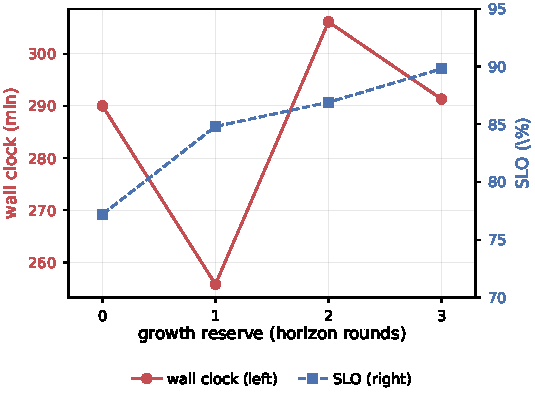
\includegraphics[width=\columnwidth]{figs/fig6_horizon.pdf}
  \caption{The growth reserve is not a free parameter. Removing it costs
  13.5\,pp of SLO; two rounds is 15 minutes slower than three. The optimum at
  one round touches the static front and does not cross it.}
  \label{fig:horizon}
\end{figure}

\section{Load Dependence}
\label{sec:load}

A negative result about adaptivity invites the obvious objection: adaptivity
pays when conditions \emph{change}, and a single stationary trace is the one
case where a static cap should be near-optimal. We agree, and we test it.

We run the same controller and the same cap family on a 25-session tier. The
throttle configuration is reversed: with all safety throttles disabled, the
25-session tier runs \emph{51\% faster} (58.4 to 28.8 minutes) at a cost of
only 2.4\,pp of SLO, while on the 200-session tier disabling the same
throttles costs 42\% (291.3 to 415.0 minutes) and 43.7\,pp of SLO. One switch,
two regimes, opposite signs, both around 40--50\%
(Fig.~\ref{fig:loadtier}). No single scalar setting is optimal across both.

This is the regime in which adaptive control should win, and we report two
findings about it. The first is discouraging for our controller: on the
25-session tier it does not win. A static cap of three, re-run under the
current harness, finishes in 24.2 minutes at 91.2\% SLO---16\% faster than the
most aggressive \sys{} configuration we measured on that tier, and with better
run-to-run stability (segment SD 5.1 against 11.0 for cap-2). The stateless
cap, which cannot see occupancy, backlog or remaining work, is simply better
here. We flag one caveat and one gap. The caveat is that the tier comparison
above is cross-generation: the 25-session throttle arms come from an earlier
harness revision and are not directly comparable to the 200-session numbers,
so we treat them as a direction rather than a magnitude. The gap is that the
matching \sys{} arm on the 25-session tier under the current harness was
interrupted by another tenant and is not reported.

The second finding is the more useful one. The signal an adaptive controller
would need is available---the number of sessions waiting for admission differs
by 6--7$\times$ between the tiers (median 9--11 at 25 sessions against 66 at
200, maximum 135)---but its \emph{interpretation} is not obvious. At the
25-session tier the controller holds eleven sessions back while running
exactly one; that backlog is manufactured by the throttling itself rather than
evidence that demand has slackened. Reading it correctly requires combining
instantaneous backlog with progress through the run, which is a stateful
computation a cap cannot perform. We regard this as the most promising
direction we did not finish, and we are explicit that we did not finish it.

\begin{figure}[tb]
  \centering
  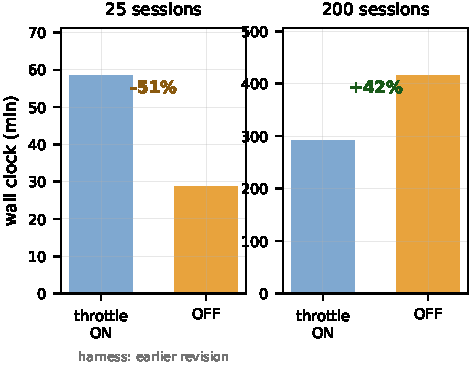
\includegraphics[width=\columnwidth]{figs/fig5_loadtier.pdf}
  \caption{The same throttle switch, two load tiers, opposite signs. The
  25-session bars are from an earlier harness revision and are shown as a
  direction, not a magnitude; the matching current-harness arm was interrupted
  and is not reported.}
  \label{fig:loadtier}
\end{figure}

\section{Related Work}
\label{sec:related}

\paragraph{Admission and scheduling for agentic serving.} Recent systems
report large gains from treating an agent session, rather than a request, as
the schedulable unit, and from preserving session state across tool calls:
session-aware admission with CPU-restorable KV
\cite{talaria,continuum}, program-level pause/resume with shortest-context-first
restoration \cite{thunderagent}, and congestion-based control over an
agent-level window \cite{concur}. A recurring measurement in this line is that
recomputation, not admission, dominates: \cite{concur} attributes 49.1\% of
end-to-end latency to recomputation, and \cite{mori} preserves state on the
CPU at the cost of a reload. Our results are consistent with this literature
rather than in tension with it, and \S\ref{sec:discussion} explains why: the
mechanism these systems add is one our controller already has.

\paragraph{Engine-side techniques.} A separate line improves the engine
rather than the admission decision. Iteration-level batching and paged KV
\cite{yu2022orca,kwon2023pagedattention} are the substrate every policy here runs
on; chunked prefill with stall-free batching \cite{sarathi}, prefill/decode
disaggregation \cite{distserve}, and cache-centric scheduling
\cite{mooncake} are the refinements. Our \S\ref{sec:model} attributes 7--10\,ms of each
26\,ms step to non-decode work, which is exactly what this line attacks. We
emphasise that these techniques raise the achievable rate for \emph{all}
policies; they move the frontier rather than deciding who sits above it.

\paragraph{State retention and preemption.} A third line keeps session state
alive across the gaps we measure in \S\ref{sec:model}: keeping KV on cheaper
storage across turns \cite{yu2025pensieve,gao2024cachedattention}, migrating it
between instances \cite{sun2024llumnix}, and preempting at iteration granularity
\cite{wu2026fastserve}. These systems exercise finer control than our 2\,s
admission cycle, which is the boundary of our negative result: we falsify one
control granularity, not the family. What they share with \sys{} is that the
state is not discarded---which is why, as we argue below, adding admission
intelligence on top buys nothing here.

\paragraph{Application-level dependencies and replay.} Serving an LLM
\emph{application} rather than a request means the scheduler sees dependencies
between calls \cite{lin2024parrot}, and agentic traces have structure that
request-level benchmarks do not capture \cite{wang2026xperf}. Our replay
preserves that structure but fixes it in advance, which is exactly the
limitation these works would press on.

\paragraph{Prefix caching.} The prefix cache is often proposed as the signal
an admission policy should use. In our workload it is not a policy variable:
round-1+ hit rate equals the trace's own planned value (89.8\%) to within one
percentage point across four different admission policies, so admission does
not move it. We note the boundary of this claim---we varied admission policy,
not eviction policy, and SGLang exposes alternate eviction policies we did not
test, and production KV-cache traces show hit rate is sensitive to policy in
ways a single trace family may not reveal \cite{wang2025kvcachewild}.

\section{Discussion}
\label{sec:discussion}

\paragraph{Why published gains do not reappear.} The systems cited above win
by preserving session state across tool waits and by pausing at agent
granularity. \sys{} inherits both properties from its permit design: a session
holds its permit for its whole lifetime and its KV is preserved across waits,
and the permit file supports the same pause primitive \cite{concur} uses. If
that mechanism is where the published gains come from---and the measurements
in those papers suggest it is---then a controller that already has it has
nothing left to add by admitting more cleverly. This reframes our negative
result: it is not that admission control cannot work, but that on this workload
the mechanism that makes it work has already been spent.

\paragraph{A criterion, not just a verdict.} The decomposition suggests a
cheap test for whether admission control can pay on a given workload. Measure
$\overline{R}$ and $\tau$ (by Method 2, which needs only per-request logs) over
a range of concurrency. If $\tau$ is flat, raising $\overline{R}$ converts
directly into wall clock and admission control has room. If $\tau$ rises
proportionally with $\overline{R}$, the two cancel and it does not. Our 13
measured configurations give 18.4--32.2\,ms across a running range of
0.64--1.62, i.e.\ a rise of 13.8\,ms over 0.98---a factor of 1.75 against a
concurrency factor of 2.5, which absorbs more than half the gain.
We offer this as the paper's constructive output, and we note it is testable
in minutes on a system that already logs per-request timings.

\paragraph{Limitations.} Our results come from one 24\,GB accelerator, one 7B
model and one trace family; generality is untested. Two specific boundaries
matter. First, the pool holds about four median sessions, so concurrency is
capacity-bound by construction; on a device with a much larger pool the
premise may not hold and the conclusion may invert---we regard reproducing on
a larger device as the single most important next experiment. Second, the
load is stationary, single-tenant and single-SLO. The load-dependence result
of \S\ref{sec:load} says the reverse should be expected when conditions vary,
and multi-tenant or heterogeneous-SLO settings are where we would look next.

\paragraph{Reproducibility.} Every verdict in this paper is produced by one
script from the raw per-step logs, and every run is guarded against a shrunken
KV pool. We report three claims we retracted during the work, because the
retractions were the most informative events: a median-based reading of the
tool wait that inverted a central assumption, a growth-sensitivity conclusion
that rested on an arm we had already invalidated, and the accounting
double-charge of \S\ref{sec:results}, falsified twice---once by source
inspection and once by the end-to-end measurement here.

\section{Conclusion}

We asked whether an adaptive admission controller can beat a tuned static
concurrency cap on a memory-bound agentic LLM workload, and found that on our
system it cannot: nine variants, four mechanistically distinct routes, none
above the static front. The reason is a cancellation. Admission policy controls
how many requests are in flight; the per-step cost rises with that number; and
the product is what the wall clock sees. We gave a two-part decomposition of
the wall clock that makes the cancellation measurable, identified a structural
idle component the policy cannot recover, and showed the regime in which
adaptivity should have paid---where the same switch is worth $+51\%$ and
$-42\%$---is one where a stateless cap still wins. The constructive output is a
per-request measurement that decides, in minutes, whether admission control
has room on a given workload.


\bibliographystyle{IEEEtran}
\bibliography{refs}

\end{document}
